\documentclass[
  letterpaper,
  twocolumn,
  9pt,
  journal,
  final]{IEEEtran}

\usepackage[spanish,es-tabla]{babel}
\usepackage[utf8]{inputenc}
\usepackage{amsfonts}
\usepackage{amsmath}
\usepackage{amssymb}
\usepackage{amsxtra}
\usepackage{mathrsfs}
\usepackage{array}
\usepackage{tikz}
\usepackage{cite}
\usepackage{varioref}
\usepackage{float}
\usepackage{color}
\usepackage{colortbl}
\usepackage{enumerate}
\usepackage{rotating}
\usepackage{subcaption}
\usepackage{hyperref}
\usepackage{listings}
\usepackage{lipsum}
%\usepackage{flushend}
\usepackage{graphicx}

\usepackage{xcolor}
\hypersetup{
    colorlinks,
    linkcolor={red!50!black},
    citecolor={blue!50!black},
    urlcolor={blue!80!black}
}



\title{Tarea 3 - Procesamiento Digital de Imágenes}
\author{\textbf{Autor:} Pablo Yáñez Santibáñez - pablo.yanez@uai.cl}
%\author{\IEEEauthorblockN{Pablo Yáñez S.} - pablo.yanez@uai.cl}

% Levels to show in table of contents:
% \setcounter{tocdepth}{-1} % only parts
% \setcounter{tocdepth}{0}  % only parts and chapters
\setcounter{tocdepth}{1}  % part,chapters,sections
% \setcounter{tocdepth}{2}  % part,chapters,sections, subsections
% \setcounter{tocdepth}{3}  % part,chapters,sections, subsections,subsubsections
% \setcounter{tocdepth}{4}  % part,chapters,sections, subsections,subsubsections and paragraphs
% \setcounter{tocdepth}{5}  % part,chapters,sections, subsections, subsubsections, paragraphs and subparagraphs.


\begin{document}
\bstctlcite{IEEEexample:BSTcontrol}
\maketitle

% \begin{abstract}
% We propose \lipsum[1]
% \end{abstract}

\tableofcontents

% \listoffigures

% \listoftables

%%%%%%%%%%%%%%%%%%%%%%%%%%%%%%%%%%%%%%%%%%%%%%%%%%%%%%%%%%%%%%%%%%%%%%%%%%%%%%%%
\section{Marco Teórico}

En el procesamiento de de señales si bien es posible realizar operaciones en el dominio del tiempo o es espacio, este tipo de operaciones tienen una alta complejidad en términos computacionales. Una alternativa para sobrellevar esto es aplicar una transformación matemática para cambiar el dominio de trabajo de la señal. En el ámbito del procesamiento de señales se utiliza la transformada de Fourier, que tiene como base la Serie de Fourier.

%%%%%%%%%%%%%%%%%%%%%%%%%%%%%%%%%%%%%%%%%%%%%%%%%%%%%%%%%%%%%%%%%%%%%%%%%%%%%%%%
\subsection{Series de Fourier - Señales Continuas}

Jean-Baptiste Joseph Fourier propuso a comienzos del Siglo XIX que cualquier función periódicas de periodo $T$ puede descomponerse en la suma infinita de funciones $sin()$ y $cos()$. La expansión en series de Fourier de una función $f(x)$ esta dada por la expresión (\ref{eq:fs}), mientras que los términos $a_0$, $a_n$ y $b_n$ se calculan según (\ref{eq:fs_a0}), (\ref{eq:fs_an}) y (\ref{eq:fs_bn}) respectivamente.




\begin{align}
	f(x) &= \frac{a_0}{2} + \sum_{n=1}^{\infty} a_n cos \left(\frac{2n\pi}{T}x\right) + \sum_{n=1}^{\infty} b_1 sin\left(\frac{2n\pi}{T}x\right) \label{eq:fs} \\
	a_0 &= \frac{1}{T} \int_{t_0}^{t_0 + T} f(x) dx \label{eq:fs_a0} \\
	a_n &= \frac{1}{T} \int_{t_0}^{t_0 + T} f(x) cos(nx) dx \label{eq:fs_an}\\
	b_n &= \frac{1}{T} \int_{t_0}^{t_0 + T} f(x) sin(nx) dx \label{eq:fs_bn}
\end{align}

Otra forma de expresar la expansion en series de Fourier de un función es utilizar la expresión en notación en exponencial, la cual se desprende al utilizar la identidad de Euler.

\begin{align}
	f(x) &= \sum_{-\infty}^{\infty} c_n e ^ {-i \frac{2\pi n}{T} x} \label{eq:fs_euler}\\
	c_N &= \frac{1}{T} \int_{t_0}^{t_0 + T} f(x) e ^ {-i \frac{2\pi n}{T} x} dx
\end{align}

Las expresiones \ref{eq:fs} y \ref{eq:fs_euler} son formas equivalentes de expresar la representación en series de Fourier de una señal periódica y real.

%%%%%%%%%%%%%%%%%%%%%%%%%%%%%%%%%%%%%%%%%%%%%%%%%%%%%%%%%%%%%%%%%%%%%%%%%%%%%%%%
\subsection{Transformada de Fourier - Señales Continuas}

La transformada de Fourier corresponde a una generalización de la serie de Fourier para señales no periódicas.
Si se tiene una función no periódica $x(t)$ como la presentada en la Figura (\ref{fig:senal_aperidica}) es posible construir una nueva señal periódica $x_p(t)$ con periodo $T_p$ repitiendo esta señal. Luego, $x(t)$ es igual a $x_p(t)$ cuando $T_p \to \infty$.

\begin{figure}[h!]
\centering
	\begin{subfigure}[b]{\columnwidth}
	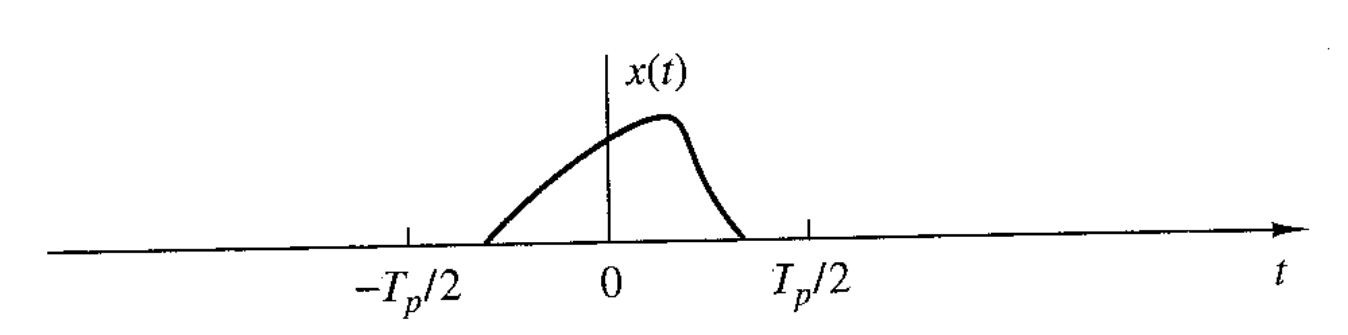
\includegraphics[width=1\linewidth, angle=-1]{imgs/proakis_aperiodic_1.png}
	\subcaption{Señal no periódicas.}
	\label{fig:senal_aperidica}
	\end{subfigure}

	\begin{subfigure}[b]{\columnwidth}
	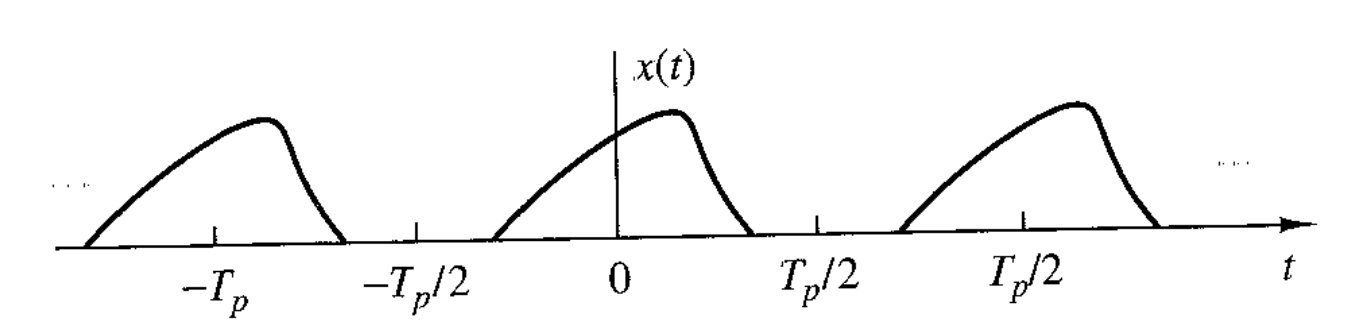
\includegraphics[width=1\linewidth, angle=-1]{imgs/proakis_aperiodic_2.png}
	\subcaption{Señal periódicas construida repitiendo (a).}
	\label{fig:senal_aperidocia_repetida}
	\end{subfigure}

\caption{Ejemplo de señal no periódicas\cite{proakis}.}
\label{fig:p4_both}
\end{figure}

El resultado de aplicar la transformada de Fourier a un función $f(x)$, cuyo dominio puede estar en el tiempo o espacio, es una función $\mathcal{F}(k)$, cuyo dominio se encuentra en el espacio de la frecuencia. En (\ref{eq:ft}) y (\ref{eq:fti}) se presenta las expresiones para el cálculo de la transformada de Fourier de una función y la de su inversa.

\begin{align}
	\mathcal{X}(F) &= \int_{-\infty}^{\infty} f(x) e^{-2\pi i F x} dt \label{eq:ft}\\
	x(t) &= \int_{-\infty}^{\infty} \mathcal{X}(F) e^{ 2\pi i F x} dF \label{eq:fti}
\end{align}

En general en la literatura es común encontrar (\ref{eq:ft}) y (\ref{eq:fti}) expresadas en función de la frecuencia angular $\omega = 2\pi F$.

\begin{align}
	\mathcal{X}(\omega) &= \int_{-\infty}^{\infty} f(x) e^{-i \omega x} dt \label{eq:ft}\\
	x(t) &= \frac{1}{2\pi} \int_{-\infty}^{\infty} \mathcal{X}(F) e^{i \omega x} d\omega \label{eq:fti}
\end{align}

\subsection{Series de Fourier - Señales Discretas}

De igual forma que una señal continua, una señal discreta $x(n)$ periódica con periodo $N$ tiene una representación en series de Fourier. La expasión en Series de Fourier se encuentra dada por (\ref{eq:dfs}), mientras que el calculo de los coeficientes de la serie se realiza utilizando (\ref{eq:dfs_coeffs}).

\begin{align}
	x(n) &= \sum_(k=0)^{N-1} c_k e^{\frac{i 2 \pi n}{N} k } \label{eq:dfs} \\
	c_k &= \frac{1}{N} \sum_(n=0)^{N-1} x(n) c_k e^{\frac{-i 2 \pi k}{N} n} \label{eq:dfs_coeffs}
\end{align}


\subsection{Transformada de Fourier - Señales Discretas}

De igual forma que en la señales continuas, es posible calcular la transformada de Fourier de una señal discreta. En (\ref{eq:dft}) y (\ref{eq:dfti}) se presentan la fórmulas para la Transforma de Fourier Discreta (DFT) y su inversa.

\begin{align}
	X(k) &= \sum_{n=0}^{N-1} x(n) e ^{-i \frac{2\pi}{N} k n } \label{eq:dft} \\
	x(n) &= \sum_{k=0}^{N-1} X(k) e ^{ i \frac{2\pi}{N} k n } \label{eq:dfti}
\end{align}

\subsection{Aplicación DFT en imagenes}

Dado que las imágenes son señales discretas en dos dimensiones para obtener su transformada de Fourier, basta con aplicarla en cada una de las dimensiones.

\begin{align}
	X(k,l) &= \sum_{i=0}^{N-1} \sum_{j=0}^{N-1} x(i,j) e ^ {-i \frac{2\pi}{N} k i} e ^ {-i \frac{2\pi}{N} l j} \label{eq:dft2} \\
	X(i,j) &= \frac{1}{N^2} \sum_{k=0}^{N-1} \sum_{l=0}^{N-1} X(k,l) e ^ {i \frac{2\pi}{N} (ki +lj)} \label{eq:dft2i}
\end{align}

En (\ref{eq:dft2}) y (\ref{eq:dft2i}) se presenta las expresiones para el cálculo de la transformada de Fourier discreta para una señal de dos dimensiones, así como la expresión para el cálculo de su inversa.


\subsection{Ruido}

En general, el ruido corresponde a una perturbación que contamina una señal. En el caso de las imágenes el ruido causa que un pixel tome un valor que no corresponde con el real.

\subsubsection{Uniforme}
produce variaciones en la imagen con una distribución de intensidades con distribución Gaussiana, afectando completamente la imagen.

\subsubsection{Impulsional}
El ruido impulsional genera valores muy altos o muy bajos, diseminado en la imagen siguiendo una distribución Gaussiana.

\subsubsection{Uniforme}
Ruido que afecta la imagen de acuerdo a una distribución uniforme, lo que produce que el histograma de la imagen se aplane. Los ruidos frecuenciales se encuentran dentro de este tipo de ruido.


\subsection{Filtrado en el dominio de la Frecuencia}

Una de las ventajas de trabajar en el espacio de la frecuencia es la posibilidad de realizar filtros en este dominio. Esto se deriva del teorema de la convolución, en el cual la operación de convolución realizada en el dominio del espacio corresponde a realizar la multiplicación de las transformadas de Fourier de ambas señales, tal como indica (\ref{eq:fft_conv}).

\begin{align}
	\begin{split}
	\mathfrak{F} (x(n) * y(n) ) &= \mathfrak{F}(x(n)) \times \mathfrak{F}(y(n))\\
	&= X(k) \times Y(k)
	\end{split}\label{eq:fft_conv}
\end{align}


Los filtros se clasifican de acuerdo a sus banda de paso.

\subsubsection{Filtro Pasa-Bajos}
Permite el paso de las componentes de baja frecuencia de la señal.

\subsubsection{Filtro Pasa-Altos}
Filtras las componentes de baja frecuencia de una señal, dejando solo las componentes de alta frecuencia.

\subsubsection{Filtro Pasa-Banda} El filtro pasa-banda solo permite el paso de las componentes de cierta banda de frecuencias.

\subsubsection{Filtro Elimina-Banda} Elimina las componentes de la señal en la banda deseada.

Si bien los filtros se exponen distintos tipos de filtros, en la práctica los filtros Pasa-Altos, Pasa-Banda y Elimina-Banda se puede construir utilizando solo filtros del tipo Pasa-Bajos.

\subsection{Filtro de Butterworth}

El filtro de Butterworth corresponde a filtro pasa-bajos diseñado para obtener una respuesta lo mas plana posible en la banda de paso. Fue presentado en 1930 por Stephen Butterworth en la publicación titulada `On the Theory of Filter Amplifiers'. En el ámbito del procesamiento de imágenes se utiliza su version 2D, cuya ecuación se presenta en (\ref{eq:Butterworth}).

\begin{align}
H(k,l) = \frac{1}{ 1 + \left(  \frac{ \sqrt{k^2 + j^2} }{f_c}  \right) ^{2N} } \label{eq:Butterworth}
\end{align}

\begin{figure}[!tbh]
  \begin{center}
    \resizebox{\columnwidth}{!}{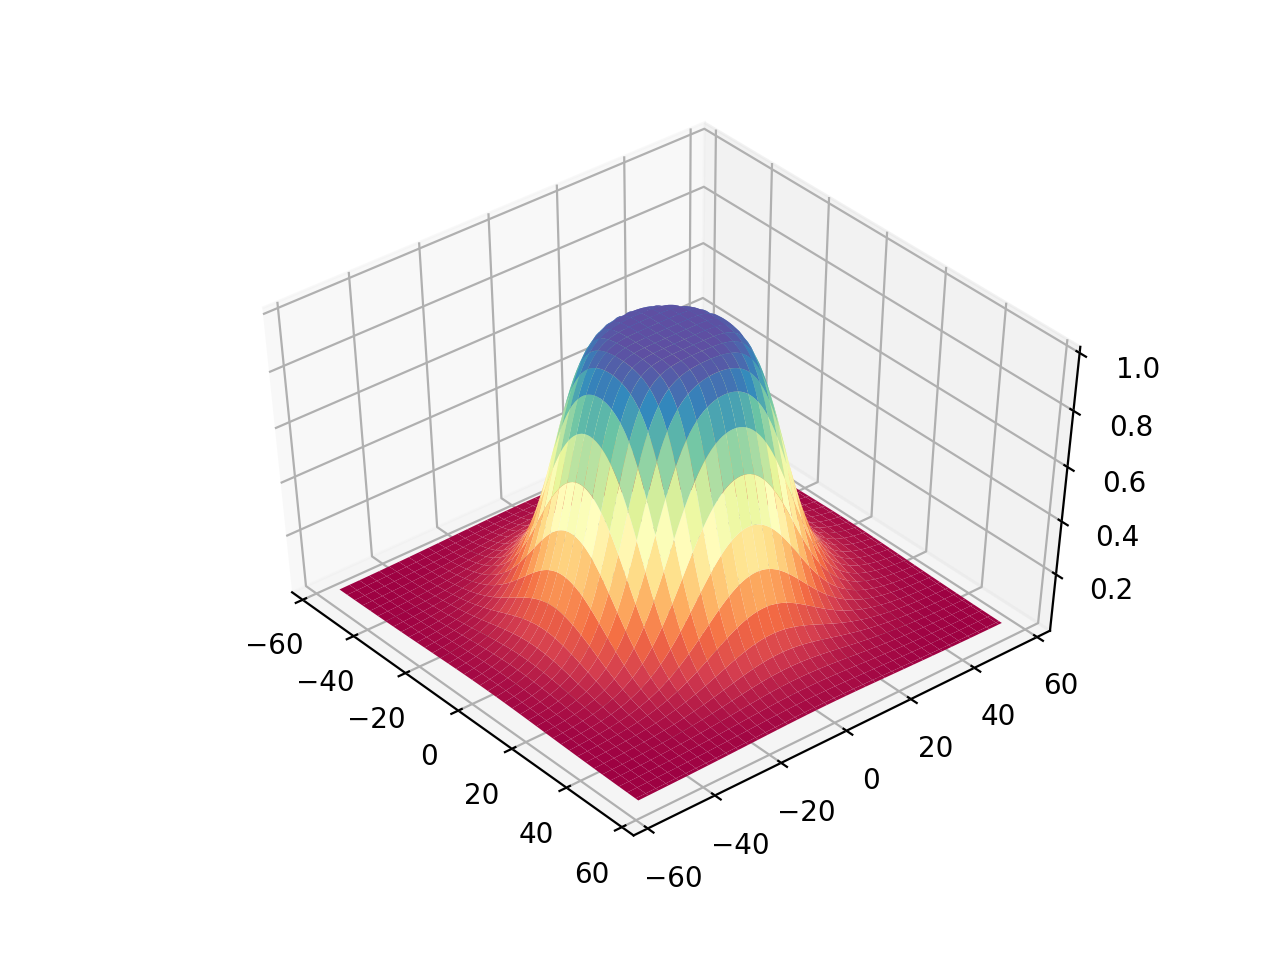
\includegraphics[trim={1cm 1cm 1cm 1cm}, clip]{butterworth_3d.png}}
  \end{center}
  \caption{Ejemplo Filtro de Butterworth 2D.} \label{fig:butter_fft}
\end{figure}

\section{Imagen a utilizar}

Se considera utilizar una fotografía realizada por \href{https://www.flickr.com/photos/carlosyanez/}{Carlos Yáñez} que se encuentra disponible en \href{https://www.flickr.com/photos/carlosyanez/29061122837/}{Flickr}. Para efectos de este trabajo solo se utiliza una sección de 512$\times$512 pixeles. El área seleccionada se presenta en la Figura (\ref{fig:roi_fft}).

\begin{figure}[!tbh]
  \begin{center}
    \resizebox{\columnwidth}{!}{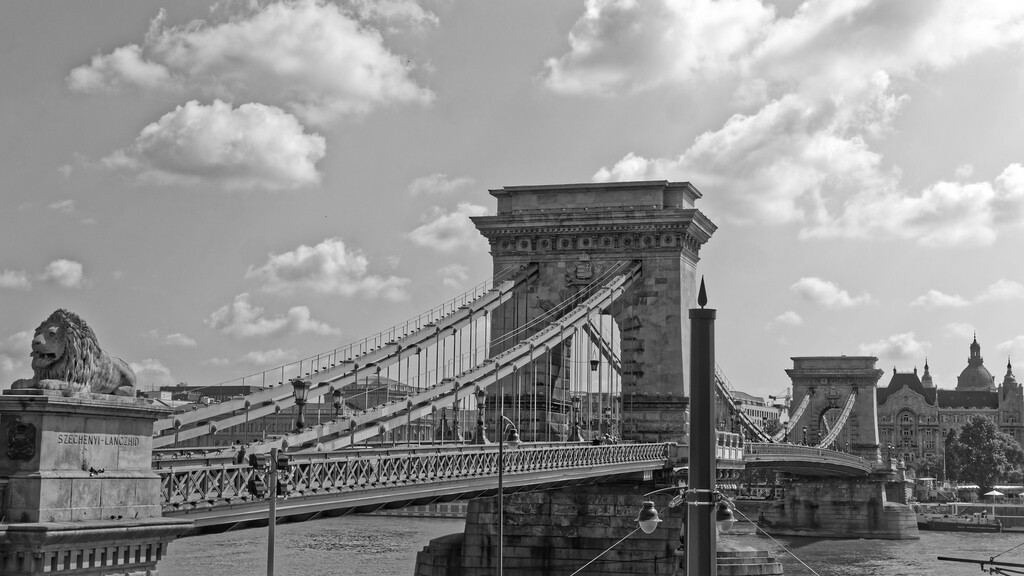
\includegraphics[]{puente.jpg}}
  \end{center}
  \caption{Fotografía de un puente.} \label{fig:original}
\end{figure}

\begin{figure}[!tbh]
  \centering
  \begin{minipage}[b]{0.49\columnwidth}
    \includegraphics[width=\textwidth, trim={0cm 0cm 0cm 0cm}, clip]{outs_1/p1/puente_roi.jpg}
    \subcaption{Sección a utilizar}
	\end{minipage}
  % \hfillz
  \begin{minipage}[b]{0.49\columnwidth}
    \includegraphics[width=\textwidth, trim={2.5cm 0.5cm 3cm 0.8cm}, clip]{outs_1/p1/puente_fft.png}
    \subcaption{Espectro}
  \end{minipage}
  \caption{Area seleccionada.} \label{fig:roi_fft}
\end{figure}


\section{Ruido Frecuencial - Generación y Filtrado}

\subsection{Generación}

Se contamina la imagen con ruido frecuencia de 10, 50 y 80 [Hz]. El resultado de aplicar ruido en estas frecuencias se puede apreciar en en la Figura \ref{fig:puente_ruido}.

\begin{figure}[!tbh]
  \centering
  \begin{subfigure}[b]{.31\linewidth}
    \includegraphics[width=\linewidth]{outs_1/p2/10/puente.jpg}
    \caption{10 [Hz]}\label{fig:hz10}
  \end{subfigure}
  \begin{subfigure}[b]{.31\linewidth}
    \includegraphics[width=\linewidth]{outs_1/p2/50/puente.jpg}
    \caption{50 [Hz]}\label{fig:hz50}
  \end{subfigure}
  \begin{subfigure}[b]{.31\linewidth}
    \includegraphics[width=\linewidth]{outs_1/p2/80/puente.jpg}
    \caption{80 [Hz]}\label{fig:hz80}
  \end{subfigure}
  \caption{Imagen contaminada con ruido frecuencial.}
  \label{fig:puente_ruido}
\end{figure}

\subsection{Filtrado}

Se considera realizar el filtrado de las imágenes en el dominio de la frecuencia. Para ello se obtiene el espectro de las tres imágenes se presenta en la Figura \ref{fig:fft_ruido_freq}.

\begin{figure}[!tbh]
	\centering

  \begin{subfigure}[b]{.3\linewidth}
    \includegraphics[width=\linewidth,trim={2.5cm 0.5cm 3cm 0.8cm}, clip]{outs_1/p2/10/puente_fft.png}
	\end{subfigure}
  \begin{subfigure}[b]{.3\linewidth}
    \includegraphics[width=\linewidth,trim={2.5cm 0.5cm 3cm 0.8cm}, clip]{outs_1/p2/50/puente_fft.png}
	\end{subfigure}
  \begin{subfigure}[b]{.3\linewidth}
    \includegraphics[width=\linewidth,trim={2.5cm 0.5cm 3cm 0.8cm}, clip]{outs_1/p2/80/puente_fft.png}
	\end{subfigure}

  \begin{subfigure}[b]{.3\linewidth}
		\begin{tikzpicture}
			\tikzset{NoBorderBox/.style={rectangle, minimum size=6mm,top color=white, align=center }}
			\tikzset{BorderBox/.style={rectangle, minimum size=12mm, rounded corners=1mm, thick,draw, top color=white, align=center}}
			\node[anchor=south west,inner sep=0] (evm) at (0,0) {\includegraphics[width=\linewidth,trim={2.5cm 0.5cm 3cm 0.8cm}, clip]{outs_1/p2/10/puente_fft_seccion.png}};
			\begin{scope}[x={(evm.south east)},y={(evm.north west)}]
			\node[circle, red, ultra thick, draw, minimum size = 5mm] (ADC) at (0.4,0.5) {};
			\node[circle, red, ultra thick, draw, minimum size = 5mm] (ADC) at (0.7,0.5) {};
			\end{scope}
			\end{tikzpicture}
	\end{subfigure}
  \begin{subfigure}[b]{.3\linewidth}
		\begin{tikzpicture}
			\tikzset{NoBorderBox/.style={rectangle, minimum size=6mm,top color=white, align=center }}
			\tikzset{BorderBox/.style={rectangle, minimum size=12mm, rounded corners=1mm, thick,draw, top color=white, align=center}}
			\node[anchor=south west,inner sep=0] (evm) at (0,0) {\includegraphics[width=\linewidth,trim={2.5cm 0.5cm 3cm 0.8cm}, clip]{outs_1/p2/50/puente_fft_seccion.png}};
			\begin{scope}[x={(evm.south east)},y={(evm.north west)}]
			\node[circle, red, ultra thick, draw, minimum size = 5mm] (ADC) at (0.22,0.5) {};
			\node[circle, red, ultra thick, draw, minimum size = 5mm] (ADC) at (0.88,0.5) {};
			\end{scope}
			\end{tikzpicture}
	\end{subfigure}
	\begin{subfigure}[b]{.3\linewidth}
		\begin{tikzpicture}
			\tikzset{NoBorderBox/.style={rectangle, minimum size=6mm,top color=white, align=center }}
			\tikzset{BorderBox/.style={rectangle, minimum size=12mm, rounded corners=1mm, thick,draw, top color=white, align=center}}
			\node[anchor=south west,inner sep=0] (evm) at (0,0) {\includegraphics[width=\linewidth,trim={2.5cm 0.5cm 3cm 0.8cm}, clip]{outs_1/p2/80/puente_fft_seccion.png}};
			\begin{scope}[x={(evm.south east)},y={(evm.north west)}]
				\node[circle, red, ultra thick, draw, minimum size = 5mm] (ADC) at (0.2,0.5) {};
				\node[circle, red, ultra thick, draw, minimum size = 5mm] (ADC) at (0.9,0.5) {};
			\end{scope}
		\end{tikzpicture}
  \end{subfigure}

  \caption{Espectro de imagenes con ruido frecuencial.} \label{fig:fft_ruido_freq}
\end{figure}

Es posible observar en la Figura \ref{fig:fft_ruido_freq} que al incorporar el ruido indicado se agregó energía en las componentes espectrales correspondientes, lo que se aprecia como puntos blancos en el espectro de las imágenes.

Para el proceso de filtrado se construye una filtro elimina-banda con frecuencias de corte $f_{c1}
= f - 1$ y $f_{c1} = f = 1$, donde $f$ corresponde a la frecuencia que utilizada para generar la señal de ruido. La Tabla \ref{tab:fc} muestra en detalle las frecuencias de corte utilizadas para cada unos de los filtros. Respecto al orden del filtro, se prueban varios valores y se elige el menor valor que presente el mejor resultado.

\begin{table}[!tbh]
\centering
\caption{Frecuencias de corte para los distintos Filtros}
\label{tab:fc}
\begin{tabular}{l | l |l | l }
$f$  & $f_{c1}$ & $f_{c2}$  & Orden\\  \hline \hline
10 & 9   & 11 & 19 \\
50 & 49  & 51 &  9 \\
80 & 79  & 81 & 19 \\
\end{tabular}
\end{table}

\begin{figure}[!tbh]
	\centering

  \begin{subfigure}[b]{.3\linewidth}
    \includegraphics[width=\linewidth,]{outs_1/p3/10/puente_N19.png}
	\end{subfigure}
  \begin{subfigure}[b]{.3\linewidth}
    \includegraphics[width=\linewidth,]{outs_1/p3/50/puente_N09.png}
	\end{subfigure}
  \begin{subfigure}[b]{.3\linewidth}
    \includegraphics[width=\linewidth,]{outs_1/p3/80/puente_N19.png}
	\end{subfigure}

  \begin{subfigure}[b]{.3\linewidth}
		\includegraphics[width=\linewidth,trim={2.5cm 0.5cm 3cm 0.8cm}, clip]{outs_1/p3/10/puente_fft_post_filter_N19.png}
		\caption{10 [Hz]}
	\end{subfigure}
  \begin{subfigure}[b]{.3\linewidth}
    \includegraphics[width=\linewidth,trim={2.5cm 0.5cm 3cm 0.8cm}, clip]{outs_1/p3/50/puente_fft_post_filter_N09.png}
		\caption{50 [Hz]}
	\end{subfigure}
  \begin{subfigure}[b]{.3\linewidth}
    \includegraphics[width=\linewidth,trim={2.5cm 0.5cm 3cm 0.8cm}, clip]{outs_1/p3/80/puente_fft_post_filter_N19.png}
		\caption{80 [Hz]}
	\end{subfigure}

  \caption{Resultado post-filtrado.} \label{fig:post-filt}
\end{figure}


En la Figura \label{fig:post} se presentan los resultados después de haber filtrado las imágenes. En todos los casos se logra eliminar satisfactoriamente el ruido.

\section{Ruido Desconocido - Generación y Filtrado}

\subsection{Generación}

De acuerdo a las instrucciones de modifica la modifica la fotografáa del hombre con la cámara. El resultado se presenta en la Figura \ref{camaraman}.

\begin{figure}[!tbh]
	\centering

  \begin{subfigure}[b]{.49\linewidth}
		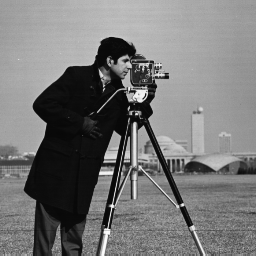
\includegraphics[width=\linewidth,]{cameraman.png}
		\caption{Original}
	\end{subfigure}
  \begin{subfigure}[b]{.49\linewidth}
    \includegraphics[width=\linewidth,]{outs_2/p1/cameraman_mod.jpg}
		\caption{Modificado}
	\end{subfigure}

  \caption{Hombre con la cámara.} \label{camaraman}
\end{figure}


\subsection{Filtrado}

Para el filtrado de esta imagen se considera el siguiente proceso:

\begin{enumerate}
	\item Aplicar Transformada de Fourier para obtener el espectro.
	\item Binarizar el espectro para identificar las zonas donde existe componentes con alto valor.
	\item Binarizar el espectro con un umbral mayor para identificar las zonas con mayor valor (que corresponde al centro del espectro).
	\item Restar ambas imágenes binarias para obtener así una plantilla que indica las zonas a filtrar.
	\item Atenuar complemente las zonas indicadas en las máscara obtenida.
	\item Aplicar la Transformada Inversa para obtener la imagen filtrada.
\end{enumerate}

El espectro de la imagen presentado en la Figura \ref{camaraman_fft} y se puede observar que el ruido agregado a la imagen tiene componentes en distintas secciones del espectro.

\begin{figure}[!tbh]
	\includegraphics[width=\linewidth,]{outs_2/p1/cameraman_mod_fft.png}
	\caption{Espectro imagen modificada.} \label{camaraman_fft}
\end{figure}

El espectro mostrado en \ref{camaraman_fft} se binariza considerando un umbral de $0.5$ y $0.75$. Luego se opera ambas imágenes para construir la máscara mostrada en la Figura \ref{mi_filtro}. Esta imagen final es la que se utiliza como filtro.

\begin{figure}[!tbh]
	\centering
  \begin{subfigure}[b]{.3\linewidth}
		\includegraphics[width=\linewidth,trim={2.5cm 0.5cm 3cm 0.8cm}, clip]{outs_2/p2/spect_bina_0.50.png}
		\caption{Treshold $0.5$}
	\end{subfigure}
  \begin{subfigure}[b]{.3\linewidth}
    \includegraphics[width=\linewidth,trim={2.5cm 0.5cm 3cm 0.8cm}, clip]{outs_2/p2/spect_bina_0.75.png}
		\caption{Treshold $0.75$}
	\end{subfigure}
  \begin{subfigure}[b]{.3\linewidth}
    \includegraphics[width=\linewidth,trim={2.5cm 0.5cm 3cm 0.8cm}, clip]{outs_2/p2/0.50_0.75_mask.png}
		\caption{Mascara Final} \label{mi_filtro}
	\end{subfigure}
  \caption{Binarización del espectro.} \label{bin_spectrum}
\end{figure}



\begin{figure}[!tbh]
	\centering
  \begin{subfigure}[b]{.49\linewidth}
		\includegraphics[width=\linewidth]{outs_2/p2/0.50_0.75_cm_0.00.png}
		\caption{Imagen}
	\end{subfigure}
  \begin{subfigure}[b]{.49\linewidth}
    \includegraphics[width=\linewidth,trim={2.5cm 0.5cm 3cm 0.8cm}, clip]{outs_2/p2/im2.png}
		\caption{Espectro}
	\end{subfigure}
  \caption{Imagen filtrada.} \label{camera_filtered}
\end{figure}

La Figura \ref{camera_filtered} presenta los resultados obtenidos al realizar el procedimiento descrito. Se aprecia que el método de filtrado no logra eliminar complemente el ruido presente en la imagen. En algunas áreas se logra eliminar gran parte de el (ej: Chaqueta), pero se debería estudiar otra técnica para filtrar esta imagen.


\section{Código}

Se adjunta dos códigos para reproducir los resultados presentados en este documento. Su ejecución se realiza según lo indicado a continuación.

\begin{verbatim}
	# Ejecuta Parte 1
	python pablo_yanez_t3_parte1.py

	# Ejecuta Parte 2
	python pablo_yanez_t3_parte2.py
\end{verbatim}





%%%%%%%%%%%%%%%%%%%%%%%%%%%%%%%%%%%%%%%%%%%%%%%%%%%%%%%%%%%%%%%%%%%%%%%%%%%%%%%%
% Bibliography
\nocite{*}
\bibliographystyle{IEEEtran}
\bibliography{bibliography}


\end{document}


% Photo:
% https://www.flickr.com/photos/carlosyanez/29061122837/



%\begin{lstlisting}[language=bash]
%  $ wget http://tex.stackexchange.com
%\end{lstlisting}

%\begin{table} \caption{A Simple Example Table} \label{table_example}
%  \begin{center}
%    \begin{tabular}{c c}
%      \hline
%      \bfseries First & \bfseries Next\\ \hline\hline
%      1.0 & 2.0 \\
%      \hline
%    \end{tabular}
%  \end{center}
%\end{table}


%\begin{lstlisting}[float=tbh!, caption={Magnitud de la respuesta en frecuencia del filtro IIR},label={cod:mag resp frec %IIR}]
%mag=20*log10(abs(H));
%\end{lstlisting}